% Figures for iaa_distinct_frequencies.hpp -- how distinct-value frequencies are
% counted on the Intel IAA without sorting and without a CPU pass over the data.
%
%   pdflatex iaa_distinct_frequency.tex
%
% Needs only pgf/tikz and geometry.

\documentclass[11pt]{article}

\usepackage[T1]{fontenc}
\usepackage[a4paper,margin=1.4cm]{geometry}
\usepackage{tikz}
\usepackage{xcolor}

\usetikzlibrary{positioning,arrows.meta,calc,fit,decorations.pathreplacing}

\definecolor{iaablue}{HTML}{1F5C8B}
\definecolor{iaagrey}{HTML}{6B7280}
\definecolor{iaalight}{HTML}{EDF2F6}
\definecolor{iaaequal}{HTML}{F4DDAF}
\definecolor{iaalow}{HTML}{C9DFEC}
\definecolor{iaahigh}{HTML}{D2E6D8}

\tikzset{
  cell/.style   ={draw=iaagrey!65, fill=white, minimum size=5.2mm, inner sep=0pt,
                  font=\small},
  eqcell/.style ={cell, fill=iaaequal},
  lowcell/.style={cell, fill=iaalow},
  hicell/.style ={cell, fill=iaahigh},
  gone/.style   ={cell, draw=iaagrey!35, fill=iaagrey!8, text=iaagrey!70,
                  font=\scriptsize},
  bit/.style    ={cell, font=\scriptsize, text=iaagrey!80},
  bitset/.style ={cell, fill=iaablue!22, font=\scriptsize\bfseries, text=iaablue},
  rlabel/.style ={anchor=east, font=\small\ttfamily, text=iaablue},
  rnote/.style  ={anchor=west, font=\footnotesize},
  dim/.style    ={anchor=west, font=\footnotesize, text=iaagrey},
  tnode/.style  ={draw=iaablue!55, fill=iaalight, rounded corners=2pt,
                  align=center, font=\scriptsize, inner sep=4pt},
  tleaf/.style  ={tnode, fill=iaaequal!45},
  tedge/.style  ={-{Stealth[length=2mm]}, draw=iaagrey, thin},
  chain/.style  ={-{Stealth[length=2mm]}, draw=iaablue!70, thick},
  brace/.style  ={decorate, decoration={brace, amplitude=4pt, raise=1.5pt},
                  draw=iaagrey},
  slotcell/.style={draw=iaablue!45, fill=iaablue!10, minimum width=1.04cm,
                   minimum height=6mm, inner sep=0pt, font=\scriptsize\ttfamily},
  emptycell/.style={draw=iaagrey!25, fill=none, minimum width=1.04cm,
                    minimum height=6mm, inner sep=0pt, font=\scriptsize,
                    text=iaagrey!60},
}

% \cellrow{style}{y}{comma list}
\newcommand{\cellrow}[3]{%
  \foreach [count=\i from 0] \val in {#3} {%
    \node[#1] at (\i*0.52,#2) {\val};%
  }%
}
% \bitrow{y}{set indices}{count-1}
\newcommand{\bitrow}[3]{%
  \foreach \i in {0,...,#3} { \node[bit] at (\i*0.52,#1) {0}; }%
  \foreach \i in {#2} { \node[bitset] at (\i*0.52,#1) {1}; }%
}

\newcommand{\op}[1]{\texttt{#1}}
\setlength{\parskip}{4pt}
\setlength{\parindent}{0pt}

\begin{document}

\begin{center}
  {\Large\bfseries Distinct-value frequencies on the Intel IAA}\\[2pt]
  {\small figures for \op{test-sort/iaa\_distinct\_frequencies.hpp}}
\end{center}

\op{scan\_eq} counts the elements of a range equal to a value the caller already
knows: QPL writes one bit per element and the completion record's
\op{sum\_value} carries the population count. That is one descriptor per
question, so a histogram would seem to need one pass over the whole range per
distinct value --- $O(n\!\cdot\!D)$, worse as cardinality grows.

The fix is to stop offering a scan elements that cannot match it. \op{select}
compacts a range through a bit mask, and a scan produces exactly such a mask, so
the accelerator partitions its own input. Every figure below uses the same
16-element range, whose 5 distinct values are counted by 5 nodes and 14
descriptors, with the CPU never comparing or moving an element.

\bigskip
\hrule
\bigskip

{\large\bfseries 1. One node: five descriptors, strictly in order}

The pivot is an element of the range, so \op{scan\_eq} is guaranteed to find it,
and its count is final the moment the descriptor retires --- that value is never
looked at again. The two masks split everything else into ranges that are
disjoint \emph{in value}.

\begin{center}
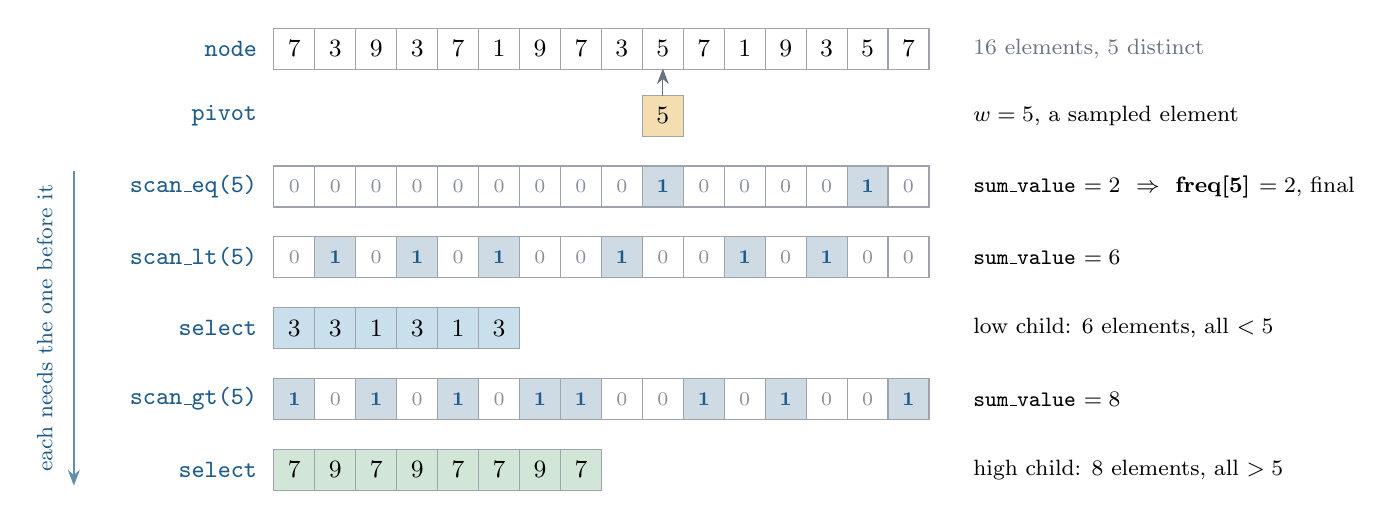
\begin{tikzpicture}
  % ---- the node -----------------------------------------------------------
  \node[rlabel] at (-0.35,0) {node};
  \cellrow{cell}{0}{7,3,9,3,7,1,9,7,3,5,7,1,9,3,5,7}
  \node[dim] at (8.5,0) {16 elements, 5 distinct};

  % pivot
  \node[rlabel] at (-0.35,-0.85) {pivot};
  \node[eqcell] at (9*0.52,-0.85) {5};
  \node[rnote] at (8.5,-0.85) {$w=5$, a sampled element};
  \draw[tedge] (9*0.52,-0.6) -- (9*0.52,-0.25);

  % ---- scan_eq ------------------------------------------------------------
  \node[rlabel] at (-0.35,-1.75) {scan\_eq(5)};
  \bitrow{-1.75}{9,14}{15}
  \node[rnote] at (8.5,-1.75)
    {\op{sum\_value} $=2$ \ $\Rightarrow$ \ \textbf{freq[5] $=2$}, final};

  % ---- scan_lt ------------------------------------------------------------
  \node[rlabel] at (-0.35,-2.65) {scan\_lt(5)};
  \bitrow{-2.65}{1,3,5,8,11,13}{15}
  \node[rnote] at (8.5,-2.65) {\op{sum\_value} $=6$};

  \node[rlabel] at (-0.35,-3.55) {select};
  \cellrow{lowcell}{-3.55}{3,3,1,3,1,3}
  \node[rnote] at (8.5,-3.55) {low child: 6 elements, all $<5$};

  % ---- scan_gt ------------------------------------------------------------
  \node[rlabel] at (-0.35,-4.45) {scan\_gt(5)};
  \bitrow{-4.45}{0,2,4,6,7,10,12,15}{15}
  \node[rnote] at (8.5,-4.45) {\op{sum\_value} $=8$};

  \node[rlabel] at (-0.35,-5.35) {select};
  \cellrow{hicell}{-5.35}{7,9,7,9,7,7,9,7}
  \node[rnote] at (8.5,-5.35) {high child: 8 elements, all $>5$};

  % ---- the dependency chain ----------------------------------------------
  \draw[chain] (-2.8,-1.55) -- (-2.8,-5.55);
  \node[text=iaablue, font=\footnotesize, rotate=90, anchor=south]
    at (-2.95,-3.55) {each needs the one before it};
\end{tikzpicture}
\end{center}

$2+6+8=16$: the pivot's copies leave the walk entirely, which is why the two
children together are shorter than their parent and the recursion terminates.

\bigskip

{\large\bfseries 2. The partition tree: one node per distinct value}

Recursing on both sides is Dijkstra's three-way partition with the equal bucket
replaced by its own population count. Nothing is sorted --- only counted. Each
node resolves exactly one distinct value, so a range with $D$ distinct values
costs at most $D$ nodes however it is ordered.

\begin{center}
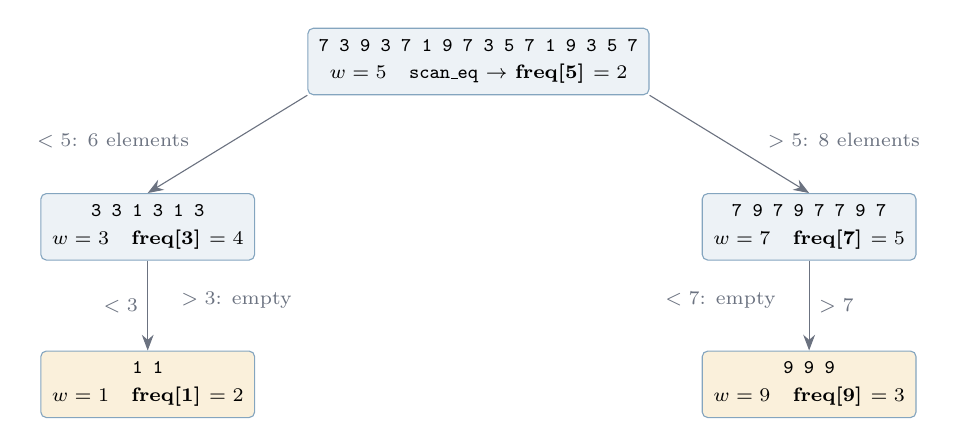
\begin{tikzpicture}
  \node[tnode] (root) at (0,0)
    {\op{7 3 9 3 7 1 9 7 3 5 7 1 9 3 5 7}\\[2pt]
     $w=5$ \ \ \op{scan\_eq} $\to$ \textbf{freq[5] $=2$}};

  \node[tnode] (a) at (-4.2,-2.1)
    {\op{3 3 1 3 1 3}\\[2pt]
     $w=3$ \ \ \textbf{freq[3] $=4$}};
  \node[tnode] (b) at (4.2,-2.1)
    {\op{7 9 7 9 7 7 9 7}\\[2pt]
     $w=7$ \ \ \textbf{freq[7] $=5$}};

  \node[tleaf] (c) at (-4.2,-4.1)
    {\op{1 1}\\[2pt] $w=1$ \ \ \textbf{freq[1] $=2$}};
  \node[tleaf] (d) at (4.2,-4.1)
    {\op{9 9 9}\\[2pt] $w=9$ \ \ \textbf{freq[9] $=3$}};

  \draw[tedge] (root.south west) -- (a.north);
  \draw[tedge] (root.south east) -- (b.north);
  \node[font=\scriptsize, text=iaagrey, anchor=east] at (-3.55,-1.0)
    {$<5$: 6 elements};
  \node[font=\scriptsize, text=iaagrey, anchor=west] at (3.55,-1.0)
    {$>5$: 8 elements};

  \draw[tedge] (a.south) -- node[left, font=\scriptsize, text=iaagrey]
    {$<3$} (c.north);
  \draw[tedge] (b.south) -- node[right, font=\scriptsize, text=iaagrey]
    {$>7$} (d.north);
  \node[font=\scriptsize, text=iaagrey, anchor=west]
    at ($(a.south)+(0.3,-0.5)$) {$>3$: empty};
  \node[font=\scriptsize, text=iaagrey, anchor=east]
    at ($(b.south)+(-0.3,-0.5)$) {$<7$: empty};

\end{tikzpicture}
\end{center}

An empty side costs no \op{select}, and a node whose \op{scan\_eq} matches
everything (shaded) is finished by that one descriptor. \textbf{5 nodes, 5
distinct values, 14 descriptors, no CPU comparison.} Descriptor count is $O(D)$
and elements read is $O(n\log D)$, the depth being that of a three-way
quicksort. The pivot is sampled by hashing the node's own coordinates, because
every fixed rule has an input shape that defeats it --- organ-pipe data hands a
median of first, middle and last element the range minimum at every level, which
degenerates straight back to $O(n\!\cdot\!D)$.

\bigskip

{\large\bfseries 3. Where the children go: two scratch buffers, ping-pong}

\op{select} cannot write into the range it reads, so a node's children are
compacted into the \emph{other} of two scratch buffers, at the offsets the parent
occupied. Both selects finish before either child is entered, so overwriting the
parent's own range is safe.

\begin{center}
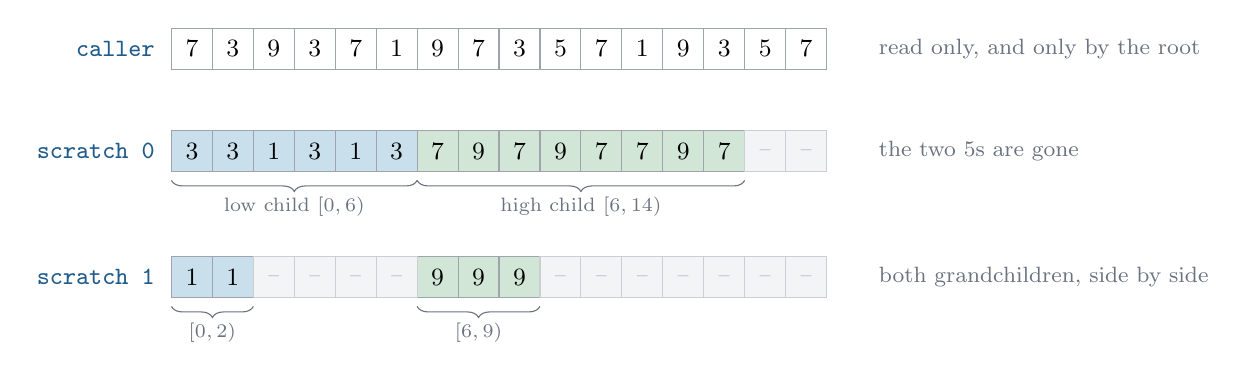
\begin{tikzpicture}
  \node[rlabel] at (-0.35,0) {caller};
  \cellrow{cell}{0}{7,3,9,3,7,1,9,7,3,5,7,1,9,3,5,7}
  \node[dim] at (8.6,0) {read only, and only by the root};

  \node[rlabel] at (-0.35,-1.3) {scratch 0};
  \cellrow{lowcell}{-1.3}{3,3,1,3,1,3}
  \foreach [count=\i from 6] \val in {7,9,7,9,7,7,9,7} {
    \node[hicell] at (\i*0.52,-1.3) {\val};
  }
  \node[gone] at (14*0.52,-1.3) {--};
  \node[gone] at (15*0.52,-1.3) {--};
  \node[dim] at (8.6,-1.3) {the two 5s are gone};

  \draw[brace] (5*0.52+0.26,-1.62) -- (-0.26,-1.62)
    node[midway, below=4pt, font=\scriptsize, text=iaagrey] {low child $[0,6)$};
  \draw[brace] (13*0.52+0.26,-1.62) -- (6*0.52-0.26,-1.62)
    node[midway, below=4pt, font=\scriptsize, text=iaagrey] {high child $[6,14)$};

  \node[rlabel] at (-0.35,-2.9) {scratch 1};
  \cellrow{lowcell}{-2.9}{1,1}
  \foreach [count=\i from 6] \val in {9,9,9} {
    \node[hicell] at (\i*0.52,-2.9) {\val};
  }
  \foreach \i in {2,3,4,5,9,10,11,12,13,14,15} {
    \node[gone] at (\i*0.52,-2.9) {--};
  }
  \node[dim] at (8.6,-2.9) {both grandchildren, side by side};

  \draw[brace] (1*0.52+0.26,-3.22) -- (-0.26,-3.22)
    node[midway, below=4pt, font=\scriptsize, text=iaagrey] {$[0,2)$};
  \draw[brace] (8*0.52+0.26,-3.22) -- (6*0.52-0.26,-3.22)
    node[midway, below=4pt, font=\scriptsize, text=iaagrey] {$[6,9)$};

\end{tikzpicture}
\end{center}

A subtree writes only inside its parent's offset range, and siblings hold
disjoint ranges. So any set of nodes containing no node together with one of its
descendants --- which is exactly what the work list holds, since children are
published only after their parent's compactions retire --- occupies pairwise
disjoint memory, and its nodes can advance at the same time. That is what makes
the next figure possible.

\medskip

{\large\bfseries 4. Pipelining: one thread, several descriptors in flight}

Within a node the five descriptors are a dependency chain, and
\op{qpl\_execute\_job} would spend one device round trip of thread time on each.
Independent nodes have no such dependency, so \op{qpl\_submit\_job} /
\op{qpl\_check\_job} carry several through their chains at once:
\op{poll()} retires whatever completed, submits what it can, and returns without
waiting.

\begin{center}
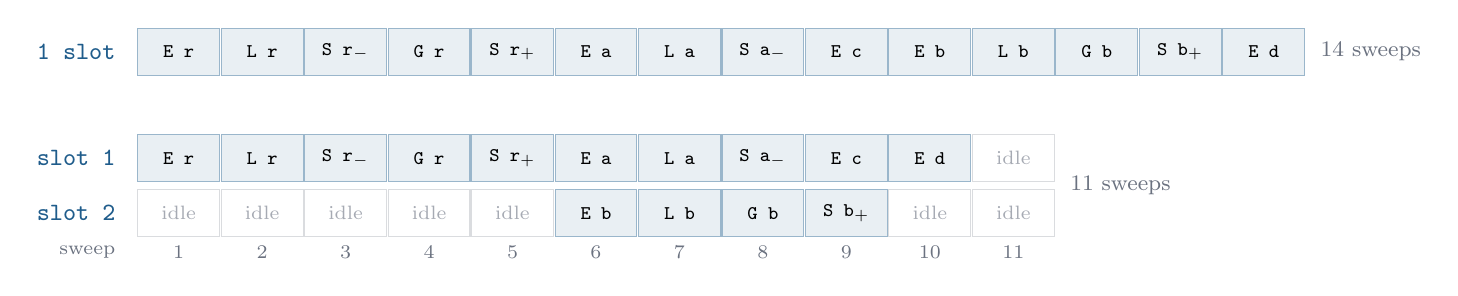
\begin{tikzpicture}
  % sequential baseline
  \node[rlabel] at (-0.68,0.5) {1 slot};
  \foreach [count=\i from 0] \d in {%
      {E r},{L r},{S r$_-$},{G r},{S r$_+$},{E a},{L a},{S a$_-$},{E c}} {
    \node[slotcell] at (\i*1.06,0.5) {\d};
  }
  \foreach [count=\i from 9] \d in {{E b},{L b},{G b},{S b$_+$},{E d}} {
    \node[slotcell] at (\i*1.06,0.5) {\d};
  }
  \node[dim] at (13*1.06+0.6,0.5) {14 sweeps};

  % pipelined
  \node[rlabel] at (-0.68,-0.85) {slot 1};
  \foreach [count=\i from 0] \d in {%
      {E r},{L r},{S r$_-$},{G r},{S r$_+$},{E a},{L a},{S a$_-$},{E c},{E d}} {
    \node[slotcell] at (\i*1.06,-0.85) {\d};
  }
  \node[emptycell] at (10*1.06,-0.85) {idle};

  \node[rlabel] at (-0.68,-1.55) {slot 2};
  \foreach \i in {0,1,2,3,4} { \node[emptycell] at (\i*1.06,-1.55) {idle}; }
  \foreach [count=\i from 5] \d in {{E b},{L b},{G b},{S b$_+$}} {
    \node[slotcell] at (\i*1.06,-1.55) {\d};
  }
  \foreach \i in {9,10} { \node[emptycell] at (\i*1.06,-1.55) {idle}; }
  \node[dim] at (10*1.06+0.6,-1.2) {11 sweeps};

  \foreach [count=\i from 0] \s in {1,2,3,4,5,6,7,8,9,10,11} {
    \node[font=\scriptsize, text=iaagrey] at (\i*1.06,-2.05) {\s};
  }
  \node[font=\scriptsize, text=iaagrey, anchor=east] at (-0.68,-2.05) {sweep};
\end{tikzpicture}
\end{center}

E~=~\op{scan\_eq}, L~=~\op{scan\_lt}, G~=~\op{scan\_gt},
S$_-$/S$_+$~=~\op{select} of the low or high side; r,\,a,\,b,\,c,\,d are the five
nodes of figure~2.

The root has no sibling, so its chain runs alone; from the second level on,
independent nodes fill the slots. The same 14 descriptors are issued either way
--- only the number of sweeps changes, and a sweep is where a hardware round trip
is waited out. The gain grows with the width of the frontier: at $n=200\,000$
and $D=4096$, measured, 12\,815 descriptors take 12\,815 sweeps on one slot and
279 on 64.

\medskip

{\large\bfseries What it costs}

Measured on 200\,000 \op{uint32} elements, QPL software path. \emph{CPU} is the
elements the CPU loads: nine pivot samples per node plus the nodes small enough
to tally directly. It never compares or moves an element --- \op{scan} compares,
\op{select} moves.

\begin{center}
\begin{tabular}{r|rrrr}
  distinct $D$ & nodes & descriptors & reads per element & CPU share of $n$\\
  \hline
  16      &     16 &      112 &  15 & 0.1\,\%\\
  256     &    256 &      878 &  35 & 1.2\,\%\\
  4\,096  & 4\,096 & 12\,819 &  57 & 18\,\%\\
  62\,493 & 45\,977 & 117\,985 &  75 & 161\,\%\\
\end{tabular}
\end{center}

Nodes track $D$ and reads track $\log D$, which is the point. The per-node CPU
sampling is $O(D)$ though, so past a few thousand distinct values it outgrows a
linear CPU pass: this is a low-cardinality operation.

\end{document}
